\clearpage

\begin{center}
    {\Large\textbf{What Reveals 3D Articulation? Learning from Motion}}

    \vspace{0.1in}
    % {\Large\textbf{\textit{Supplementary Material}}}
    {{\textit{Supplementary Material}}}

    \vspace{0.1in}
    % Anonymous project page: \url{}

\end{center}

\section{Related Work}
\label{sec:supp_related_work}


We provide a comparison table of related works as shown in~\Cref{tab:related_articulation}.
\begin{table}[ht]
\centering
\small
\setlength{\tabcolsep}{2.5pt} % 稍微收缩列间距，防止表格过宽
\renewcommand{\arraystretch}{1.2} % 增加行高，让表格更有呼吸感
\resizebox{\linewidth}{!}{%
\begin{tabular}{@{}l ccccc | cccccc c | c @{}}
\toprule
& \multicolumn{5}{c|}{\textbf{Input Modality}} & \multicolumn{7}{c|}{\textbf{Output Properties}} & \textbf{Inf.} \\
\cmidrule(lr){2-6} \cmidrule(lr){7-13}
\textbf{Method} & \faAlignLeft & \faCamera & \faProjectDiagram & \textbf{3D} & \faLayerGroup & \faBoxOpen & \textbf{3D} & \faShapes & \faProjectDiagram & \faLongArrowAltRight & \faArrowsAltV & $\mathbf{1}^{+}$ & \textbf{Time} \\
\midrule

% --- 第一类：基于优化的方法 ---
\rowcolor{tableblue} \multicolumn{14}{l}{\textit{Optimization-based Methods}} \\
PARIS \cite{liu2023paris} & -- & \checkmark & -- & -- & 2 & -- & \checkmark & \checkmark & \checkmark & \checkmark & \checkmark & -- & N/A \\
AIM \cite{ai2026aim}& -- & \checkmark & -- & \checkmark & 2 & -- & \checkmark & \checkmark & \checkmark & \checkmark & \checkmark & \checkmark & N/A \\

\midrule
% --- 第二类：基于学习的方法 ---
\rowcolor{tableblue} \multicolumn{14}{l}{\textit{Learning-based Methods}} \\
GEOPARD \cite{Goyal_2025_ICCV} & -- & -- & -- & \checkmark$^\dagger$ & 1 & -- & \checkmark & -- & \checkmark & \checkmark & -- & \checkmark & N/A \\
MeshArt \cite{gao2025meshart} & -- & (\checkmark)$^o$ & -- & (\checkmark)$^o$ & 0 & \checkmark & \checkmark & \checkmark & -- & \checkmark & \checkmark & \checkmark & N/A \\
PARTICULATE \cite{li2025particulate} & -- & -- & -- & \checkmark & 1 & -- & \checkmark & \checkmark & \checkmark & \checkmark & \checkmark & \checkmark & \textasciitilde10s \\
URDF-Anything \cite{li2025urdfanything} & \checkmark & \checkmark & -- & \checkmark & 1 & -- & \checkmark & \checkmark & \checkmark & \checkmark & \checkmark & \checkmark & N/A \\

\midrule
% --- 第三类：基于检索的方法 ---
\rowcolor{tableblue} \multicolumn{14}{l}{\textit{Generation-based Methods}} \\
SINGAPO \cite{liusingapo} & -- & \checkmark & -- & -- & 1 & \checkmark & (\checkmark)$^\ast$ & \checkmark & \checkmark & \checkmark & \checkmark & \checkmark & \textasciitilde10s \\
CAGE \cite{liu2024cage} & \checkmark & -- & \checkmark & -- & 1 & \checkmark & (\checkmark)$^\ast$ & \checkmark & \checkmark & \checkmark & -- & \checkmark & N/A \\
Kinematify \cite{wang2025kinematify} & (\checkmark)$^o$ & (\checkmark)$^o$ & -- & -- & (1)$^o$ & -- & \checkmark & \checkmark & \checkmark & \checkmark & -- & \checkmark & \textasciitilde20m \\
Articulate-Anything \cite{le2024articulate} & \checkmark & (\checkmark)$^o$ & -- & -- & (1$^{+}$)$^o$ & -- & (\checkmark)$^\ast$ & \checkmark & \checkmark & \checkmark & \checkmark & -- & \textasciitilde10m \\
FreeArt3D \cite{chen2025freeart3d} & -- & \checkmark & \checkmark & -- & 6 & -- & \checkmark & \checkmark & \checkmark & \checkmark & -- & -- & \textasciitilde10m \\
Articulate AnyMesh \cite{qiu2025articulate} & -- & -- & -- & \checkmark & 1 & -- & \checkmark & \checkmark & \checkmark & \checkmark & \checkmark & \checkmark & N/A \\
DreamArt \cite{lu2025dreamart} & -- & \checkmark & -- & -- & 1 & -- & \checkmark & \checkmark & -- & \checkmark & \checkmark & -- & N/A \\
URDF-Anything+ \cite{wu2026urdfanything_plus}& -- & \checkmark & -- & \checkmark & 1 & -- & \checkmark & \checkmark & \checkmark & \checkmark & \checkmark & \checkmark & N/A  \\ 
ArtiLatent \cite{chen2025ArtiLatent} & -- & (\checkmark)$^o$ & -- & -- & (1)$^o$ & -- & \checkmark & \checkmark & \checkmark & \checkmark & \checkmark & \checkmark & \textasciitilde30s \\
ArtFormer \cite{Su_2025_CVPR} & \checkmark & (\checkmark)$^o$ & -- & -- & (1)$^o$ & \checkmark & \checkmark & \checkmark & \checkmark & \checkmark & \checkmark & \checkmark & N/A \\


\midrule
% --- 你的方法 ---
\rowcolor{blue!15} \textbf{Ours} & -- & -- & -- & \checkmark & 2 & -- & \checkmark & \checkmark & \checkmark & \checkmark & \checkmark & \checkmark & \best{\textasciitilde10s} \\
\bottomrule
\end{tabular}%
}
\caption{
\textbf{Related work overview on articulated object modeling.} 
We summarize input modalities, the number of observed articulation configurations, and output properties for various methods. 
Icons represent: 
\faAlignLeft\ Text, 
\faCamera\ Vision(e.g., image or video), 
\faProjectDiagram\ Kinematic Chain, 
\textbf{3D} Geometry(e.g., mesh or point cloud), 
\faLayerGroup\ Number of observed articulation configurations. 
State counts are modality-agnostic: image, video, mesh, and point-cloud observations are counted by articulation configuration.
0 denotes generation without an observed object state; $(\cdot)^o$ denotes optional conditioning, e.g., $(1)^o$ for one optional state and $(1^+)^o$ for one or more optional states.
Output columns show: 
\faBoxOpen\ BBox, 
\textbf{3D} Geometry(e.g., mesh or point cloud), 
\faShapes\ Segmentation, 
\faProjectDiagram\ Structure, 
\faLongArrowAltRight\ Axis, 
\faArrowsAltV\ Range, 
$\mathbf{1}^{+}$ Multi-joint support.
($^\ast$) denotes retrieval-based geometry. 
($^o$) indicates optional conditional inputs or outputs. 
($^\dagger$) requires pre-segmented geometry.
N/A indicates the inference time is not reported in the original paper.
}
\label{tab:related_articulation}
\end{table}


\section{Implementation Details}
\label{sec:supp_details}

\subsection{Data Processing}
\label{sec:supp_data_processing}

We preprocess articulated assets from URDF and USD sources into a unified representation for two-state articulation learning. The pipeline first converts articulated objects into normalized meshes with part-level motion annotations, then samples point clouds from the exported meshes to cache training supervision.

\paragraph{URDF processing.}
For URDF assets, we parse each object's kinematic tree and mesh references, then export two canonical articulation states. Each processed object is written to an object-level directory, where \texttt{pos\_000} corresponds to the all-zero joint state and \texttt{pos\_001} corresponds to the all-one joint state. For each state, the links are transformed by forward kinematics and merged into a single mesh. We filter out invalid assets that contain no valid mesh, only one articulated part, or more than the maximum allowed number of parts. In our preprocessing, we set this maximum to 16.
% 
To keep the two states geometrically comparable, we compute a shared normalization transform over all exported states of the same object and apply it consistently to every posed mesh. The same normalization is applied to motion annotations: prismatic ranges are scaled, and revolute or prismatic axes are shifted into the normalized coordinate frame.

\paragraph{USD processing.}
For USD assets, we follow the same output convention while extracting articulation information from USD physics joints. We traverse the USD stage, identify revolute, prismatic, and fixed joints, recover parent-child link relationships, and compute each joint axis and anchor in world coordinates. We then solve forward kinematics for the two articulation states, export each posed mesh, and save the same metadata files as in the URDF pipeline.
% 
The USD pipeline also normalizes all generated states of an object jointly. After all posed meshes are exported, we compute a shared object-level center and scale, rewrite the normalized OBJ files, and transform the saved Plucker axes and motion ranges accordingly. 

\paragraph{Point sampling and cached supervision.}
After mesh export, we cache point-level supervision from each normalized mesh. For each mesh, we sample surface points with their normals and assign them to the articulated parts using the vertex-to-part labels. To better preserve geometric discontinuities between parts, training samples combine uniformly sampled surface points with points sampled near sharp edges. If no sharp edges are detected, the sampler falls back to uniform surface sampling.
% 
For training, each cached point cloud stores the sampled point cloud, normals, point-to-part labels, a binary indicator for sharp-edge samples, the part hierarchy, and per-part motion annotations.
% 
This cached representation removes the need to repeatedly load articulated meshes during training and provides a unified supervision format across URDF- and USD-derived objects.

\subsection{Training Loss Details}
\label{sec:supp_loss_details}

For cycle consistency, we enforce that the Siamese branch produces symmetric predictions. Given the reserve-order states as input, we hope the network produces part segmentation results that are consistent with those of the forward-order branch, but with opposite articulation motion. Therefore, we first swap the order of part segmentation results in the reverse branch from $\{\hat{M}_{r}^{(s_1)},\hat{M}_{r}^{(s_0)}\}$ to $\{\hat{M}_{r}^{(s_0)},\hat{M}_{r}^{(s_1)}\}$, matching the corresponding segmentation masks in forward branch.
Then we maintain the axis of articulation motion and flip the predicted revolute range and prismatic range from $\alpha_r = \{\alpha_{\min}, \alpha_{\max}\}, l_r = \{l_{\min}, l_{\max}\}$ to $\dot{\alpha}_r = \{\alpha_{\max}, \alpha_{\min}\}, \dot{l}_r = \{l_{\max}, l_{\min}\}$, representing opposite motion.
In this way, the model faithfully learns the underlying physical laws hidden in state changes.


\section{Additional Experimental Results}
\label{sec:supp_additional_experiments}

\paragraph{Additional Ablations.}
We provide additional ablation results under two evaluation protocols.
The no-penalty protocol reports part-wise metrics after matching predicted and ground-truth parts without penalizing unmatched parts, while the penalty protocol assigns penalties to unmatched predictions or missing ground-truth parts.
Reporting both protocols helps separate two effects: how well a model aligns the parts it finds and whether it recovers all functional parts required for a complete articulated asset.

\begin{table}[!htbp]
    \centering
    \caption{\textbf{Additional ablation results without unmatched-part penalty.}
    We use the same ablation variants and metrics as in the main ablation table, but compute the part-wise metrics without penalizing unmatched predicted or ground-truth parts.}
    \label{tab:supp-ablation-without-penalty}
    \renewcommand{\arraystretch}{1.2}

    \begin{tabular*}{\linewidth}{@{\extracolsep{\fill}} l ccc ccc c @{}}
        \toprule
        \multirow{2}{*}{\textbf{Method}}
        & \multicolumn{3}{c}{\textbf{Rest state}}
        & \multicolumn{3}{c}{\textbf{Articulated state}}
        & \multirow{2}{*}{\textbf{Inf. Time}} \\
        \cmidrule(lr){2-4} \cmidrule(lr){5-7}
        & gIoU$\uparrow$ & PC$\downarrow$ & mIoU$\uparrow$
        & gIoU$\uparrow$ & PC$\downarrow$ & OC$\downarrow$
        & \\
        \midrule

        \multicolumn{8}{l}{\underline{\textbf{Single branch}}} \\
        \textbf{1-state}
        & 0.470 & 0.028 & 0.536 & 0.457 & 0.087 & 0.008 & 7s \\

        \textbf{2-state}
        & 0.545 & 0.023 & 0.580 & 0.530 & 0.077 & 0.004 & 10s \\
        
        \textbf{4-state}
        & {0.576} & {0.020} & {0.611} & {0.560} & {0.041} & {0.004} & {15s} \\

        \textbf{8-state}     
        & {0.577} & {0.019} & {0.627} & {0.598} & {0.039} & {0.004} & {18s} \\

        \textbf{w/o attn. mask}
        & 0.567 & 0.024 & 0.602 & 0.561 & 0.084 & 0.007 & 10s \\

        \midrule
        \multicolumn{8}{l}{\underline{\textbf{Siamese}}} \\

        \textbf{w/o cycle loss}
        & 0.583 & 0.020 & 0.619 & 0.567 & 0.074 & 0.005 & 10s \\

        \textbf{final model}
        & 0.578 & 0.027 & 0.617 & 0.560 & 0.075 & 0.004 & 10s \\

        \bottomrule
    \end{tabular*}
\end{table}

\begin{table}[!htbp]
    \centering
    \caption{\textbf{Additional ablation results with unmatched-part penalty.}
    This table follows the main ablation protocol, where unmatched predicted or ground-truth parts are penalized in the part-wise metrics.
    The values are copied from the main ablation table for easier side-by-side comparison with \cref{tab:supp-ablation-without-penalty}.}
    \label{tab:supp-ablation-with-penalty}
    \renewcommand{\arraystretch}{1.2}

    \begin{tabular*}{\linewidth}{@{\extracolsep{\fill}} l ccc ccc c @{}}
        \toprule
        \multirow{2}{*}{\textbf{Method}}
        & \multicolumn{3}{c}{\textbf{Rest state}}
        & \multicolumn{3}{c}{\textbf{Articulated state}}
        & \multirow{2}{*}{\textbf{Inf. Time}} \\
        \cmidrule(lr){2-4} \cmidrule(lr){5-7}
        & gIoU$\uparrow$ & PC$\downarrow$ & mIoU$\uparrow$
        & gIoU$\uparrow$ & PC$\downarrow$ & OC$\downarrow$
        & \\
        \midrule

        \multicolumn{8}{l}{\underline{\textbf{Single branch}}} \\
        \textbf{1-state}
        & {0.305} & {0.096} & {0.480} & {0.293} & {0.144} & {0.008} & {7s} \\

        \textbf{2-state}
        & {0.396} & {0.083} & {0.531} & {0.382} & {0.127} & {0.004} & {10s} \\

        \textbf{4-state}
        & {0.440} & {0.074} & {0.565} & {0.424} & {0.092} & {0.004} & {15s} \\

        \textbf{8-state}     
        & {0.456} & {0.073} & {0.574} & {0.447} & {0.088} & {0.004} & {18s} \\
        \textbf{w/o attn. mask}
        & {0.386} & {0.093} & {0.540} & {0.371} & {0.134} & {0.007} & {10s} \\ 

        \midrule
        \multicolumn{8}{l}{\underline{\textbf{Siamese}}} \\

        \textbf{w/o cycle loss}
        & {0.419} & {0.085} & {0.560} & {0.403} & {0.127} & {0.005} & {10s} \\

        \textbf{final model}
        & {0.462} & {0.074} & {0.578} & {0.445} & {0.112} & {0.004} & {10s} \\

        \bottomrule
    \end{tabular*}
\end{table}


\paragraph{Additional Visualizations.}

We provide additional visualizations in~\Cref{fig:supp_results} and in the video attached to the supplementary folder.

\subsection{Failure Case Analysis}
\label{sec:supp_failure_case}

\begin{figure}[t]
  \centering
  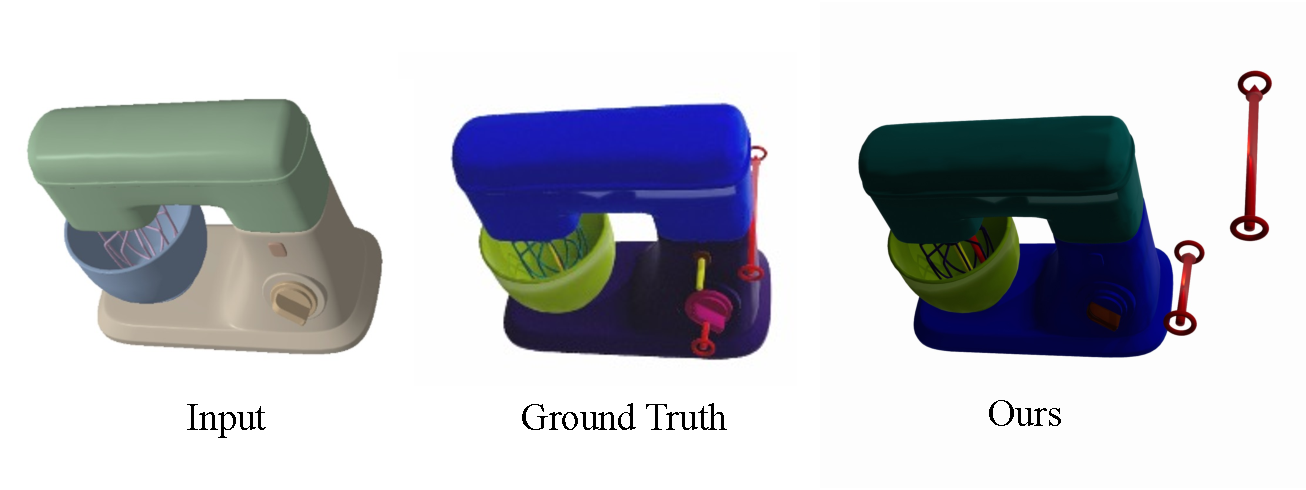
\includegraphics[width=\textwidth]{figs/failure_case.pdf}
  \caption{We show one failure case on a hierarchical object with multiple coupled rotation axes.}
  \label{fig:failure_case}
\end{figure}

\begin{figure}[t]
  \centering
  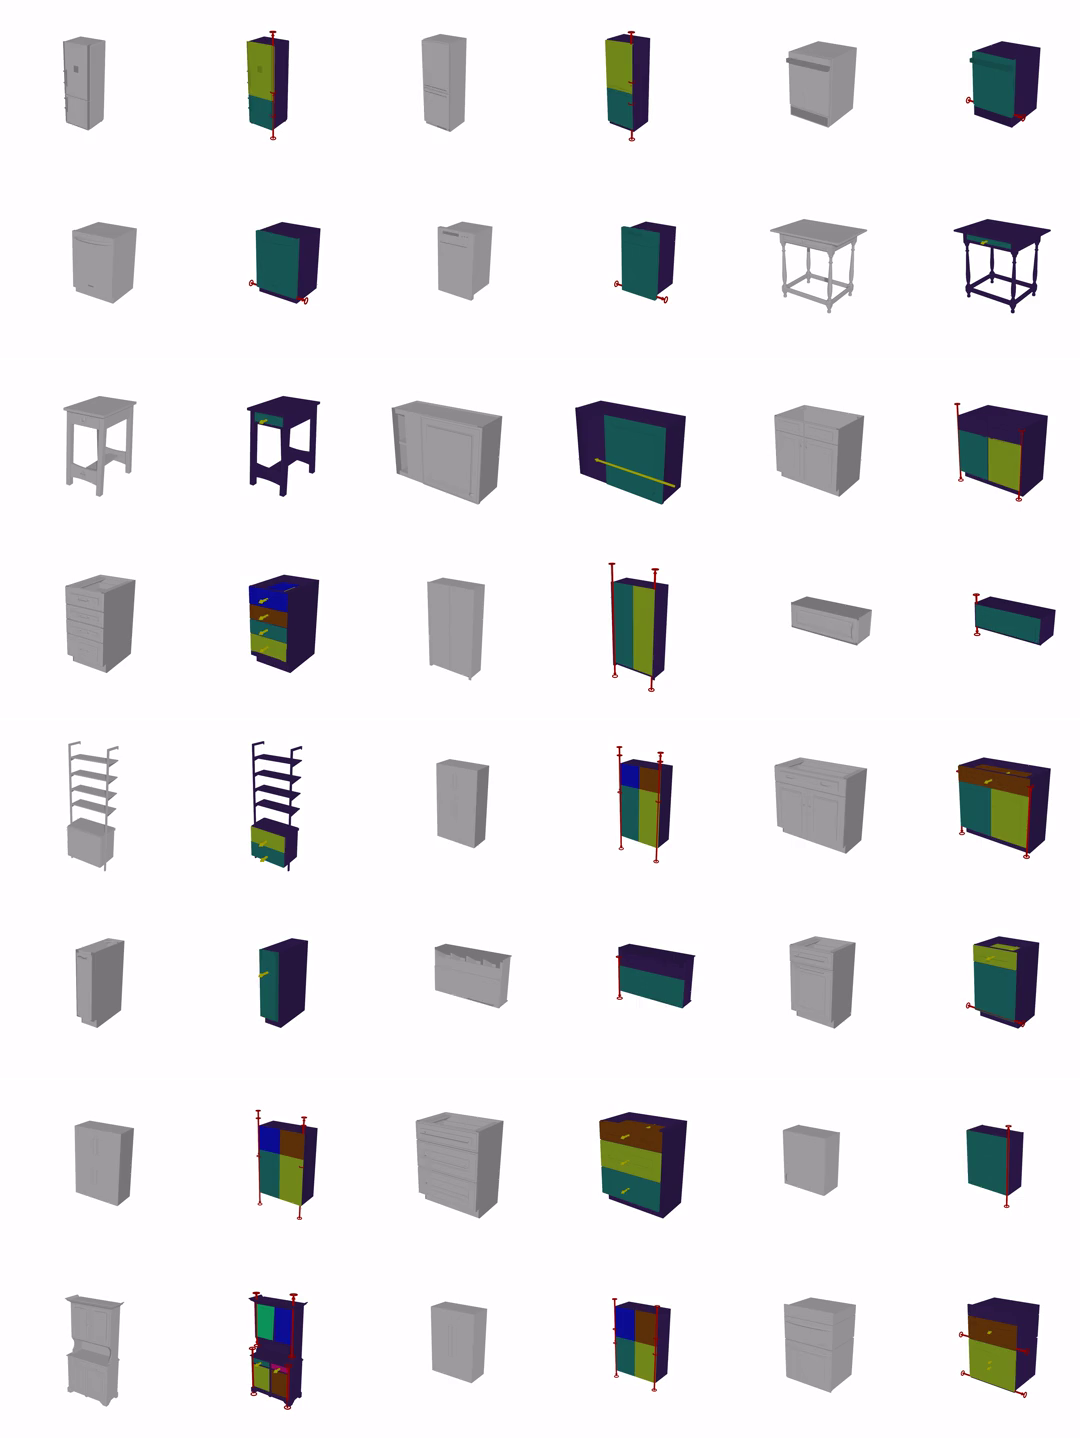
\includegraphics[width=\textwidth]{figs/supp_results.png}
  \caption{We show more visualization examples on the test set of PartNet-Mobility. Plus, we provide a video version to vividly demonstrate the articulation motion.}
  \label{fig:supp_results}
\end{figure}


A representative failure mode of \method occurs on hierarchical objects with multiple coupled rotation axes, as shown in~\Cref{fig:failure_case}.
In these cases, the motion of a child part cannot be explained by an independent joint in a fixed global frame: the child joint axis is itself transformed by the motion of its parent link.
When the parent joint rotates, the coordinate frame in which the child joint is defined also rotates, so the observed displacement of the child part is a composition of the parent motion and the child's own local articulation.
Such configurations are relatively rare in our current training data, making it difficult for a feed-forward model to learn a reliable prior for this form of nested kinematic dependency.

This failure mode is also sensitive to error accumulation along the predicted kinematic tree.
If the parent edge is assigned an inaccurate motion type, axis, pivot, or range, the resulting parent transform changes the reference frame used to interpret all descendant joints.
The child prediction must then compensate for both its own articulation error and the residual error inherited from the parent, which can produce substantially larger deviations after forward kinematic actuation than the per-joint prediction error would suggest.
Therefore, although two-state geometry provides strong evidence for ordinary articulated motion, deeply coupled multi-axis structures remain challenging when the training distribution contains few comparable examples and when small upstream errors propagate to downstream parts.

\section{Limitations.}
Our current formulation assumes that the two observations depict the same object under compatible states and that the target articulation can be represented by a tree-structured URDF.
The method may struggle when the two states differ due to severe reconstruction artifacts, non-rigid deformation, missing geometry, or contacts that hide the moving component.

\section{Statistical Reporting and Impact}
\label{sec:supp_impl_compute_impact}

\paragraph{Statistical reporting.}
For all experimental results, we report a single run under the evaluation protocol.
All reported metrics are computed on the same evaluation split for a given benchmark, and ablations change only the stated model component or training objective.

\paragraph{Broader impact.}
\method can help convert observed or generated articulated objects into simulation-ready assets, benefiting robotics, embodied AI, and virtual-environment construction.
At the same time, incorrect articulation predictions can lead to unreliable simulated interactions, especially if generated assets are used for downstream robot policy training without validation.
We therefore view the predicted URDF assets as candidates that should be checked in simulation before deployment on physical robots, and we encourage users to preserve provenance information for generated or converted assets.

